% !TeX spellcheck = en_US
\addsection{Map Elements}{\skills/logistics.png}

\begin{multicols*}{2}
Each Scenario is built using four types of Map Tiles.
Players start on their Faction-Specific Starting (I) Tile.
Other tiles may be placed and discovered as described on the next page.
During the game's setup, all face-down tiles should be selected randomly from the pool of possible Tiles as described by the Scenario and shuffled, keeping them face-down.\par
The \textbf{roman numeral} on each tile describes the overall \textbf{difficulty of Neutral Units} on that tile, as well as the number of rewards players can expect to find on that Tile.
Starting (I) Tiles are the easiest while Center (VI–VII) Tiles are the most difficult.\par

\vfill
\begin{center}
  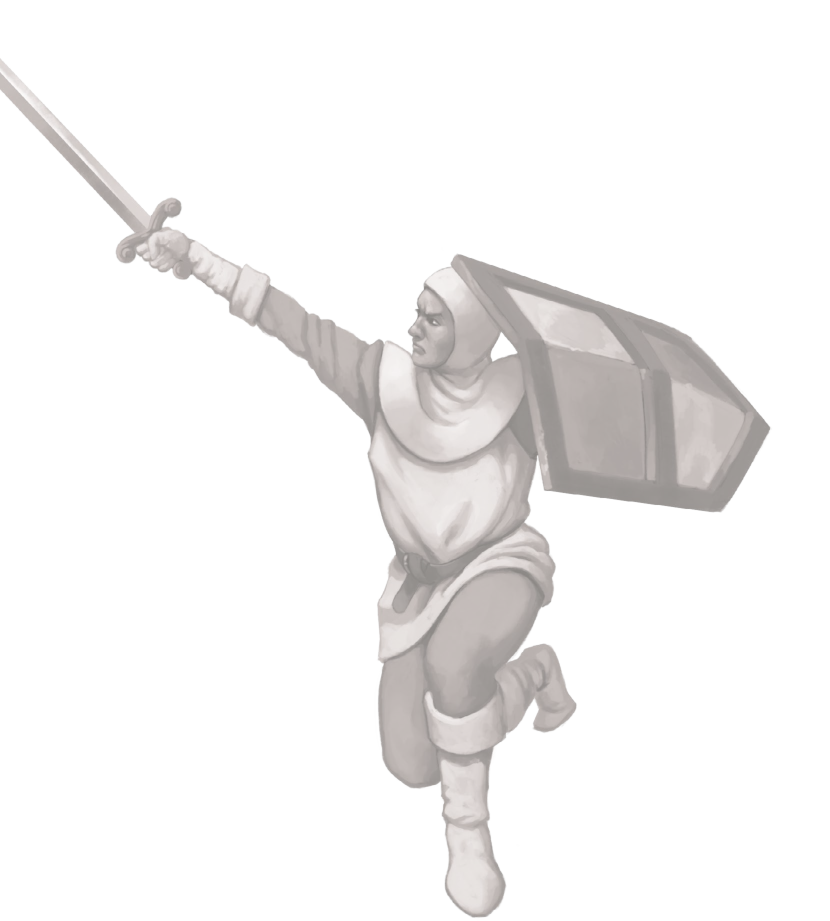
\includegraphics[width=0.7\linewidth]{\art/counterstrike.png}
\end{center}
\vfill

\subsection*{Map Tile Anatomy\index{Map Tile}}
Each Map Tile is divided into 7 separate \textbf{Fields} that your Heroes can \textbf{Visit}.
When your Hero moves to a Field, they must immediately Visit it, or
first start a \hyperlink{Combat}{Combat} against the enemies guarding it before Visiting.
Empty Fields\index{Empty Field} do nothing when Visited.
Solid yellow lines on a Field's edge cannot be passed through.
\hyperlink{Difficulty}{Roman numerals} written on a Field indicate that the Field is guarded by Neutral enemies that must be fought to Visit it.\par
\columnbreak
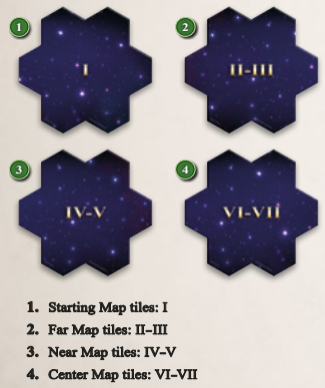
\includegraphics[width=\linewidth]{\images/maptiles.png}
\begin{itemize}
  \footnotesize
  \item[\textbf{1.}] Starting Map Tiles: I
  \item[\textbf{2.}] Far Map Tiles: II-II
  \item[\textbf{3.}] Near Map Tiles: IV-V
  \item[\textbf{4.}] Center Map Tiles: VI-VII
\end{itemize}

\vfill
\begin{center}
  \begin{scriptsize}
  \begin{tikzpicture}
    \draw (0, 0) node[inner sep=0] {\makebox[\linewidth][c]{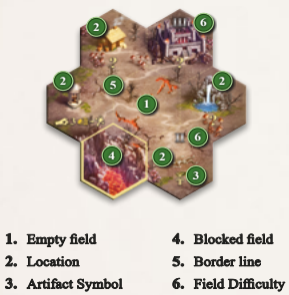
\includegraphics[width=0.75\linewidth]{\images/fields.png}}};
    \draw (0, -0.3) node {\encircle{\phantom{.}1\phantom{.}}};
    \draw (-1.9, 0) node {\encircle{\phantom{.}2\phantom{.}}};
    \draw (2.3, 0) node {\encircle{\phantom{.}2\phantom{.}}};
    \draw (-1.4, 1.7) node {\encircle{\phantom{.}2\phantom{.}}};
    \draw (0.6, -1.9) node {\encircle{\phantom{.}2\phantom{.}}};
    \draw (0.5, 1.7) node {\encircle{\phantom{.}2\phantom{.}}};
    \draw (1.4, -2.2) node {\encircle{\phantom{.}3\phantom{.}}};
    \draw (1.4, 2.5) node {\encircle{\phantom{.}4\phantom{.}}};
    \draw (1.4, -1) node {\encircle{\phantom{.}4\phantom{.}}};
    \draw (-1, 0.5) node {\encircle{\phantom{.}5\phantom{.}}};
    \draw (-1.1, -1.1) node {\encircle{\phantom{.}6\phantom{.}}};
    \draw (-1.4, -1.7) node {\encircle{\phantom{.}7\phantom{.}}};
  \end{tikzpicture}
  \end{scriptsize}
\end{center}

\begin{itemize}
  \footnotesize
  \begin{multicols}{2}
    \item[\textbf{1.}] Empty Field
    \item[\textbf{2.}] Location
    \item[\textbf{3.}] Artifact Symbol
    \item[\textbf{4.}] Field Difficulty
    \item[\textbf{5.}] Border line
    \item[\textbf{6.}] Blocked Field
    \item[\textbf{7.}] Tile name like \\{} \texttt{F2} or \texttt{\#N3}
  \end{multicols}
\end{itemize}
\end{multicols*}

\clearpage

\begin{multicols}{2}

\subsection*{\hypertarget{Categories}{Location Categories}}
Visiting Fields provides Heroes with benefits, such as gaining Resources or Cards (see \hyperlink{All Map Locations}{All Map Locations}).
There are three categories of Fields:
\begin{itemize}
  \item \textbf{Visitable} – Once you Visit this field, place a Black Cube on it.
    Treat it as an Empty Field as long as it has a Black Cube.
  \item \textbf{Flaggable} – These Fields can be captured by players and provide passive benefits.
    When you Visit one, place your Faction Cube on it.
    Enemy Heroes who Visit your Flagged Fields will replace your Cube with theirs to \textbf{steal} the Field’s effects.
    Allied Heroes treat Flagged Fields \textbf{as if they were empty}.
  \item \textbf{Revisitable} – You can Visit this Field multiple times.
    Do not place any Cubes when you Visit it.
    You may pay 1 MP to Visit this Field again.
\end{itemize}

\subsection*{\hypertarget{Placing}{Placing and Discovering New Tiles}}\index{Discovering Tiles}
Heroes may spend 1 MP to either reveal an adjacent face-down Tile, or to place a Far (II–III) Map Tile from their own supply of Tiles.
All face-down Tiles should be kept \textbf{hidden from all players} until they are about to be placed or revealed.
New tiles must be placed adjacent to the Hero who spends the MP, and connected to at least two other existing Tiles.
New Tiles must also be positioned so that there is a valid path that eventually connects them with all other Tiles.
You may always rotate Map Tiles when placing or revealing them.

\medskip
\note{6}{
  When you Visit a Visitable field, \textbf{you must} place a black cube on that Field even if you cannot or choose not to use that Field's effects.
}

\end{multicols}

\begin{figure*}[!hb]
  \centering
  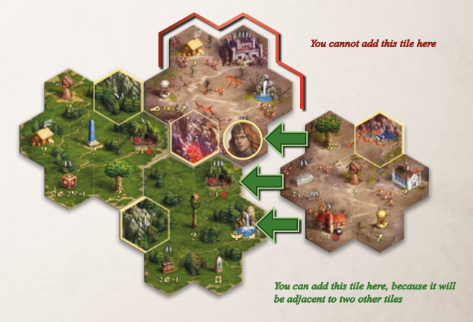
\includegraphics[width=\textwidth]{\images/placement.png}
  \begin{tikzpicture}[overlay]
    \node at (5, 10) {\footnotesize{\textbf{\textit{\textcolor{darkcandyapplered}{You cannot add this tile here}}}}};
    \node at (5, 1.4) {\footnotesize{\textbf{\textit{\textcolor{cadmiumgreen}{You can add this tile here, because it will}}}}};
    \node at (3.9, 1) {\footnotesize{\textbf{\textit{\textcolor{cadmiumgreen}{be adjacent to two other tiles}}}}};
  \end{tikzpicture}
\end{figure*}

\clearpage

\subsection*{Example Turn}

\begin{multicols*}{2}

\textit{Alice wants to capture an adjacent \hyperlink{Mines}{Mine} by Flagging it with her Main Hero, Sandro the Necromancer.
    She spends 1 MP to move onto the Mine, which begins \hyperlink{Combat}{Combat} against Neutral Units, since the Field has a \hyperlink{Difficulty}{Difficulty Rating} and has not been previously Flagged by any player.}\par

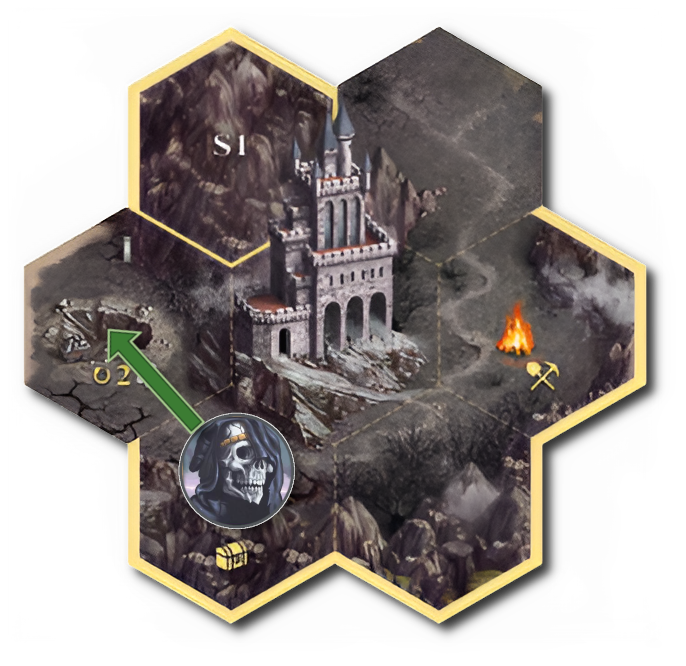
\includegraphics[width=1.1\linewidth]{\examples/sandro_takes_mine.png}

\textit{The Mine turns out to be guarded by Troglodytes, which have 3 HP \includesvg[height=0.8\baselineskip]{\svgs/health_points.svg}.
Alice's current hand consists of a Power Card, a Lightning Bolt, Haste, and a Town Portal.
During the Combat, she casts the Lightning Bolt, and Empowers \includesvg[height=0.8\baselineskip]{\svgs/empower.svg} it with Haste's alternative (bottom) effect, which makes the Lightning Bolt deal 3 damage \includesvg[height=0.8\baselineskip]{\svgs/damage.svg}, killing the Troglodytes and winning the Combat.}

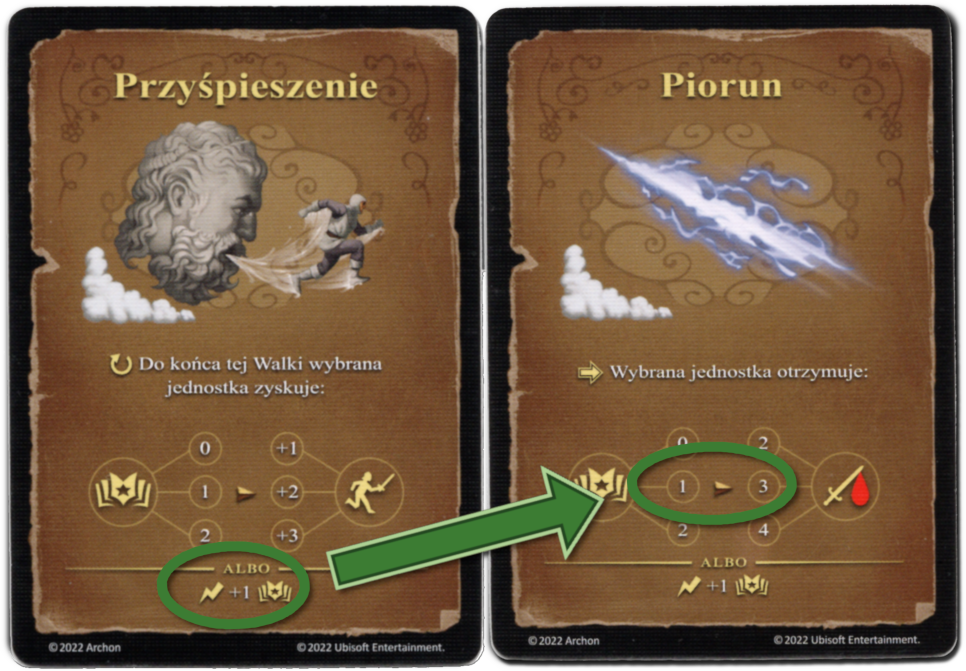
\includegraphics[width=\linewidth]{\examples/sandro_empowering_lightning_bolt.png}

\textit{The Combat lasted for only one Round, so Alice would not have been able to cast both Lightning Bolt and Haste, since players are limited to playing only one Spell Card per Combat Round.}\par


\textit{Alice now Flags the Mine by placing one of her Faction Cubes on it.
    Flagging this particular Mine increases her Building Materials \includesvg[height=0.8\baselineskip]{\svgs/building_materials.svg} production by 2, and she also immediately gains the Mine's production value of 2 \includesvg[height=0.8\baselineskip]{\svgs/building_materials.svg} as she was the first player to Flag it.}\par
\textit{Afterwards, Alice wants to go back to defend a previously Flagged Settlement by casting the Town Portal still left in her hand.
    Her Hero is Level 2, so she can empower it with the Power Card's Expert Effect \includesvg[height=0.8\baselineskip]{\svgs/expert.svg}, which grants her an additional Movement Point after casting it.
}

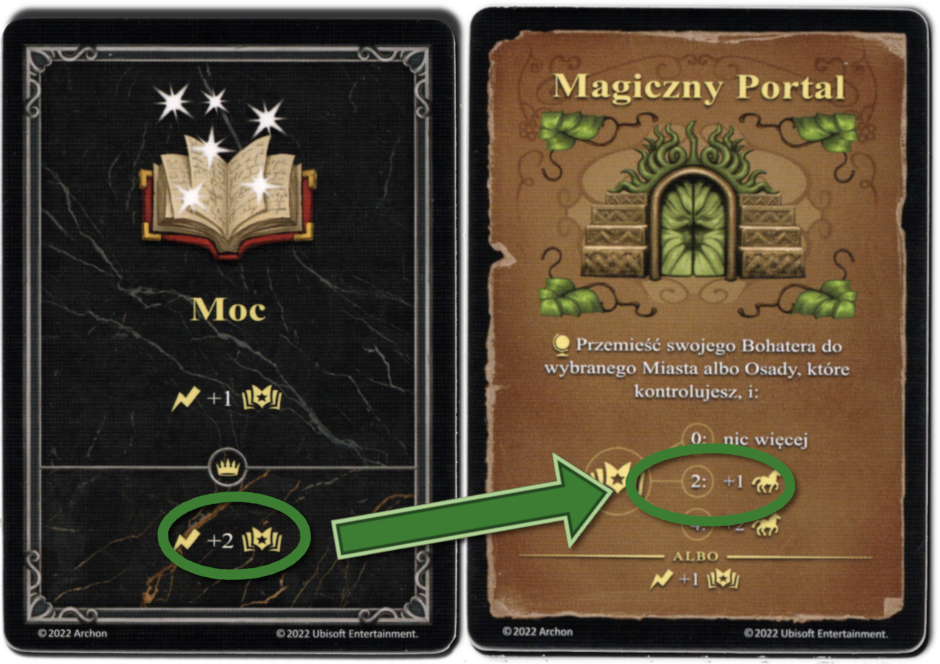
\includegraphics[width=\linewidth]{\examples/sandro_empowering_town_portal.png}

\vfill
\hspace{2em}
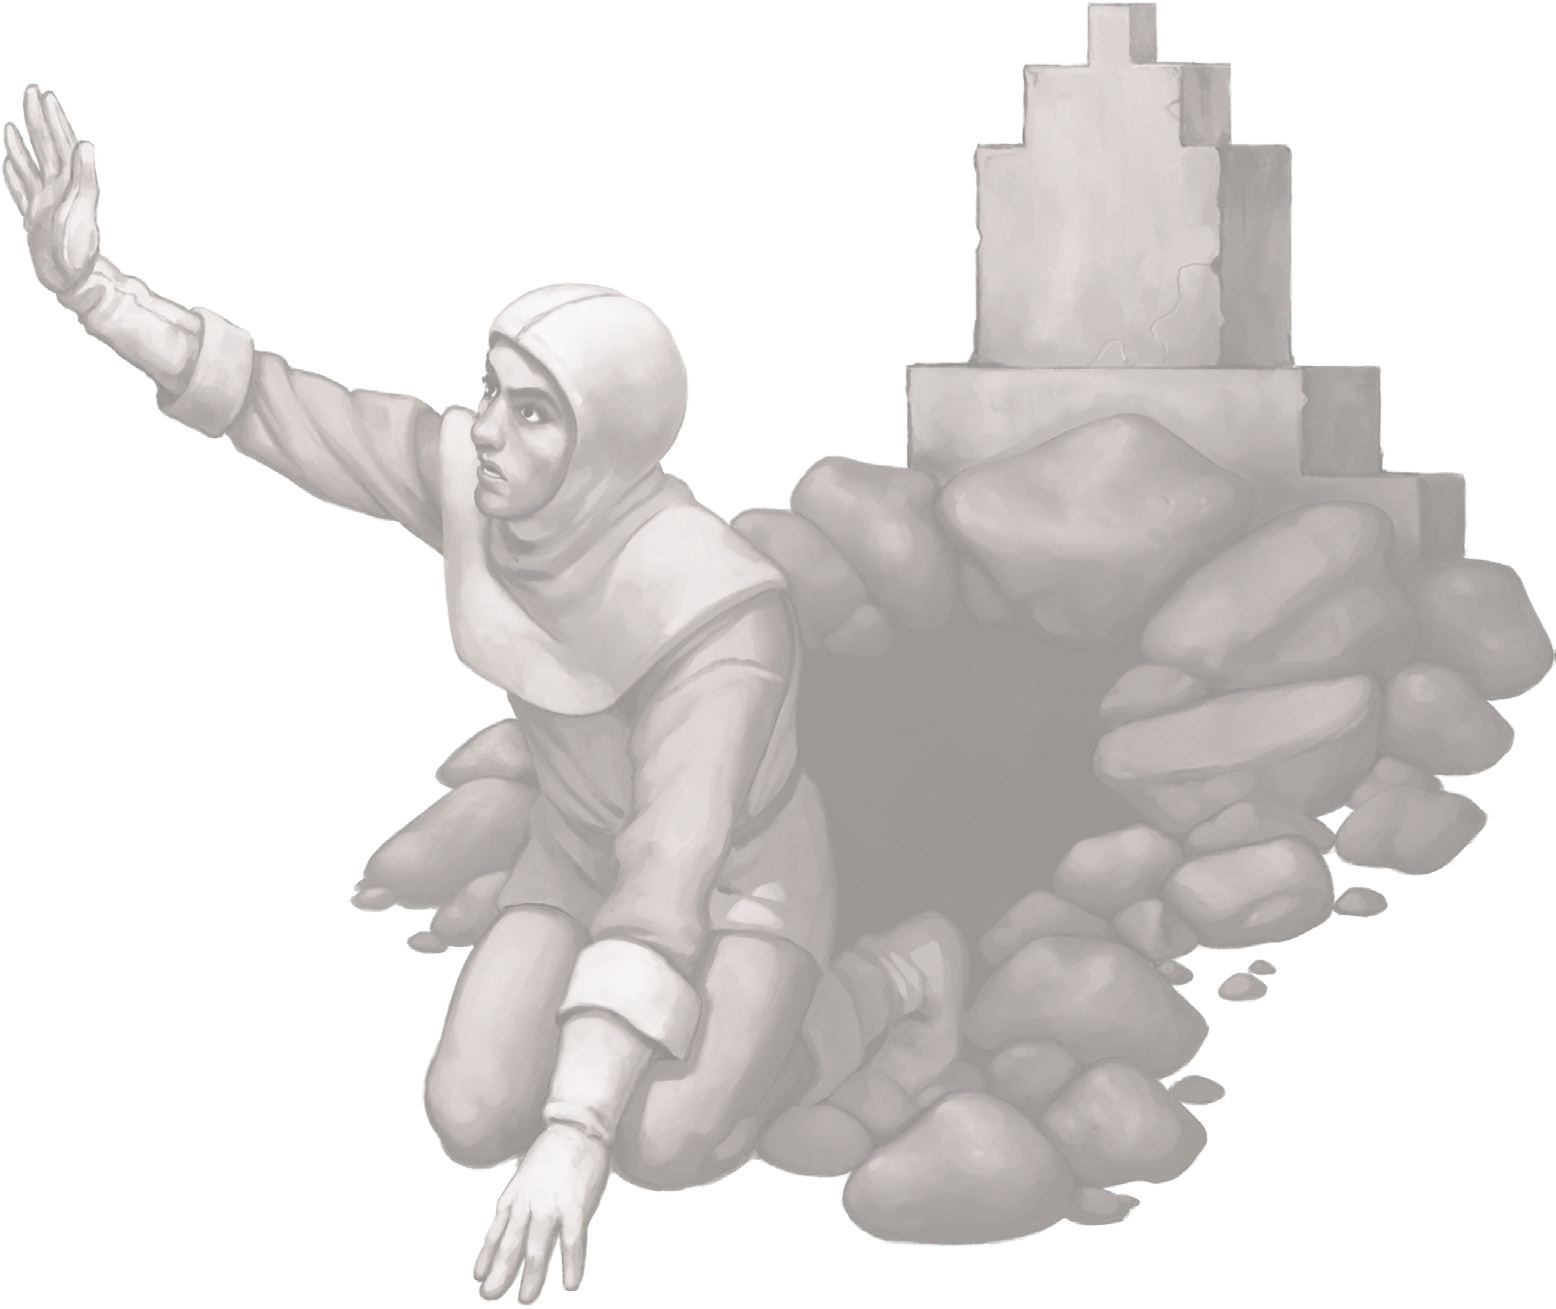
\includegraphics[width=\linewidth]{\art/resurrection.png}
\end{multicols*}
